\documentclass[handout]{beamer}
\usepackage{amsmath,amssymb,amsthm,array}
\usepackage{bm}
\usepackage{multirow}
\usepackage{multicol}
\usepackage{algorithm}
\usepackage{hyperref}
\usepackage{algorithmic}
\usepackage[normalem]{ulem}
\usepackage{fontspec}
\usepackage{numprint}
\usepackage{verbatim}
\usepackage{bm} 
\usepackage{listings}

\usetheme{Berlin}
\usecolortheme{beaver}

\setbeamertemplate{navigation symbols}{}
\title{zk-SNARKs}
\author{Panagiotis Grontas}
\date{01/06/2017}
\defbeamertemplate*{footline}{shadow theme}
{%
  \leavevmode%
  \hbox{\begin{beamercolorbox}[wd=.5\paperwidth,ht=2.5ex,dp=1.125ex,leftskip=.3cm plus1fil,rightskip=.3cm]{author in head/foot}%
    \usebeamerfont{author in head/foot}\insertframenumber\,/\,\inserttotalframenumber\hfill  (\insertshortinstitute)
  \end{beamercolorbox}%
  \begin{beamercolorbox}[wd=.5\paperwidth,ht=2.5ex,dp=1.125ex,leftskip=.3cm,rightskip=.3cm plus1fil]{title in head/foot}%
    \usebeamerfont{title in head/foot}\insertshorttitle%
  \end{beamercolorbox}}%
  \vskip0pt%
}
\institute{NTUA}
 
 \hypersetup{
  pdfauthor={Panagiotis Grontas},
  pdftitle={zk-Snarks},
  colorlinks=true,
  urlcolor=blue,
  linkcolor=white
}

\setlength{\columnseprule}{0.4pt}
\begin{document}
 
\newcommand{\xor}{ \oplus }
\newcommand{\msg}{ \mathtt{M} }
\newcommand{\KEY}{ \mathtt{K} }
\newcommand{\prv}{$\mathcal{P}$ }
\newcommand{\ver}{$\mathcal{V}$ }
\newcommand{\siml}{$\mathcal{S}$ }
\newcommand{\CPH}{ \mathtt{C} }
\newcommand{\keygen}{\mathtt{KeyGen}}
\newcommand{\enc}{\mathtt{Enc}}
\newcommand{\dec}{\mathtt{Dec}}
\newcommand{\sign}{\mathtt{Sign}}
\newcommand{\verify}{\mathtt{Verify}}
\newcommand{\adv}{$\mathcal{A}$}
\newcommand{\Hash}{\mathcal{H}}
\newcommand{\advb}{$\mathcal{B}$}
\newcommand{\chal}{$\mathcal{C}$}
\newcommand{\cs}{$\mathcal{CS}$}
\newcommand{\Zed}{\mathbb{Z}} 
\newcommand{\zns}{\mathbb{Z}^*_n}
\newcommand{\zs}[1]{\mathbb{Z}^*_{#1}}

\newcommand{\green}[1]{\textcolor{teal}{#1}}
\newcommand{\Green}[1]{\textcolor{Teal}{#1}}
\newcommand{\ForestGreen}[1]{\textcolor{ForestGreen}{#1}}
\newcommand{\blue}[1]{\textcolor{blue}{#1}}
\newcommand{\magenta}[1]{\textcolor{magenta}{#1}}
\newcommand{\cyan}[1]{\textcolor{cyan}{#1}}

\newcommand{\twopartdef}[4]
{ 
		\begin{cases}
			#1 , #2 \\
			#3 , #4
		\end{cases} 
}

\newcommand\pythonstyle{\lstset{
language=Python,
basicstyle=\ttm,
otherkeywords={self},             % Add keywords here
keywordstyle=\ttb\color{deepblue},
emph={MyClass,__init__},          % Custom highlighting
emphstyle=\ttb\color{deepred},    % Custom highlighting style
stringstyle=\color{deepgreen},
frame=tb,                         % Any extra options here
showstringspaces=false            % 
}}

\lstnewenvironment{python}[1][]
{
\pythonstyle
\lstset{#1}
}
{}

% Python for external files
\newcommand\pythonexternal[2][]{{
\pythonstyle
\lstinputlisting[#1]{#2}}}

% Python for inline
\newcommand\pythoninline[1]{{\pythonstyle\lstinline!#1!}}


\begin{frame}
\titlepage
\end{frame}

\section{Introduction}
\begin{frame}{From theory to practice...}
\begin{block}{zkSnark}
\textbf{Z}ero \textbf{K}nowledge \textbf{S}uccinct \textbf{N}on \textbf{I}nteractive \textbf{A}rguments Of \textbf{K}nowledge
\end{block}

\begin{block}{Use}
Efficiently verify the correctness of computations without executing them
\end{block}

\begin{block}{Applications}
\begin{itemize}
    \item Verify cloud computations (centralised, decentralised)
    \item Anonymous bitcoin (ZCash)
\end{itemize}
\end{block}
\end{frame}

\begin{frame}{Application Model}
\begin{itemize}
    \item A client owns input $u$ (e.g query)
    \item A server owns a private input $w$ (e.g. private DB)
    \item The client wishes to learn $z=f(u,w)$ for a function $f$ known to both
    \item Client: computation correctness (integrity)
    \item Server: private input confidentiality
\end{itemize}
Client: its computing power should be confined to the bare minimum of sending $u$ and receiving $z$
\end{frame}

\begin{frame}{What zk-Snarks offer}
\begin{itemize}
    \item \textbf{Z}ero \textbf{K}nowledge: The client (verifier \ver) learns nothing but the validity of the computation
    \item \textbf{S}uccinct: The proof is tiny compared to the computation 
    \begin{itemize}
        \item the proof size is constant $O_{\lambda}(1)$ (depends only on the security parameter $\lambda$)
        \item verification time is $O_{\lambda}(|f| + |u| + |z|)$ and does not depend on the running time of $f$
    \end{itemize}
    \item \textbf{N}on \textbf{I}nteractive: The proofs are created without interaction with the verifier and are publicly verifiable strings
    \item \textbf{A}rguments: Soundness is guaranteed only against a computationally bounded server (prover \prv)
    \item of \textbf{K}nowledge: The proof cannot be constructed without access to a witness
\end{itemize}
\end{frame}

\begin{frame}{Position in the complexity landscape...}
    \begin{itemize}
        \item $NP = PCP[O(logn),O(1)]$
        \item $NP \subseteq ZK$ (Goldreich, Micali, Wigderson)
        \item We can use PCP to construct ZK proofs (in theory)
        \item The proofs are hugely inefficient
        \item Can we construct better SNARKs without using PCPs?
        \item Yes, using QSPs and QAP - a better characterisation of NP and cryptographic assumptions
    \end{itemize}
\end{frame}

\begin{frame}{Main idea} 
\begin{enumerate}
\item Transform the verification of the computation to checking a relation between \emph{secret} polynomials: 
\begin{align*}\textrm{computation validity} \leftrightarrow p(x)q(x)=s(x)r(x) \end{align*}
\item The verifier chooses a random evaluation point that must be kept \emph{secret}: 
\begin{align*} p(x_0)q(x_0)=s(x_0)r(x_0) \end{align*}
\item Homomorphic Encryption to compute the evaluation of the polynomials at $x_0$ by using $\enc(x_0)$:
\begin{align*}\enc(p(x_0))\enc(q(x_0))=\enc(s(x_0))\enc(r(x_0))
\end{align*}
\item Blinding for ZK:
\begin{align*}
\enc(p(x_0))\enc(q(x_0)) k =\enc(s(x_0))\enc(r(x_0)) k 
\end{align*}
\end{enumerate}

\end{frame}

\section{Prerequisites}

\subsection{ZK Proofs}

\begin{frame}{ZK Proofs}
\begin{itemize}
\item Shaffi Goldwasser, Silvio Micali and Charles Rackoff, 1985
\pause
\item Interactive proof systems
\pause
\begin{itemize}
\item Computation as a dialogue
\pause
\item Prover (\prv): wants to prove that a string belongs to a language
\pause
\item Verifier (\ver): wants to check the proof st: 
\pause
\begin{itemize}
\item A correct proof convinces \ver with overwhelming probability
\item A wrong proof convinces \ver with negligible probability
\end{itemize}
\end{itemize}
\item Zero Knowledge Proofs
\begin{itemize}
\item \ver is convinced without learning anything else
\end{itemize}
\pause
\end{itemize}
A breakthrough with many theoretical and practical applications
\end{frame}

\begin{frame}{\textit{\href{http://mathoverflow.net/questions/22624/example-of-a-good-zero-knowledge-proof}{An easy example}}}
\begin{itemize}
\item \ver is color blind
\pause
\item O \prv holds two identical balls of different color
\pause
\item Can the \ver be convinced of the different colors? 
\pause
\item \green{Yes}
\begin{itemize}
\item \prv hands the balls to \ver (\green{commit})
\item \ver hides the balls behind his back, one in each hand
\pause
\item He \green{randomly} decides to switch hands or not
\pause
\item \ver presents the balls to \prv (\green{challenge})
\pause
\item \prv responds if the balls have switched hands (\green{response})
\pause
\item \ver accepts or not
\pause
\item Malicious \prv: Cheating Probability $50\%$
\pause
\item \green{Repeat} to reduce
\end{itemize}
\end{itemize}
\end{frame}

\begin{frame}{Definitions: Notation}

\begin{itemize}
\item Language $ \mathcal{L} \in \mathtt{NP}$
\item Polynomial Turing Machine $\mathcal{M}$
\item $x \in \mathcal{L} \Leftrightarrow \exists w \in \{0,1\}^{p(|x|)}: M(x,w) = 1$
\item 2 PPT TM \prv, \ver
\item $<\mathcal{P}(x,w), \mathcal{V}(x)>$ is the interaction between  \prv, \ver with common public input $x$ and private \prv input $w$.
\item $out_\mathcal{V}{<\mathcal{P}(x,w), \mathcal{V}(x)>}$ is the output of \ver at the end of the protocol
\end{itemize}
\end{frame}


\begin{frame}{Properties: Completeness and Soundness}
\begin{block}{Completeness}
An honest \prv, convinces an \emph{honest} \ver with certainty:
If  $x \in \mathcal{L}$ and $M(x,w) = 1$ then:
$ Pr[out_{\mathcal{V}}<\mathcal{P}(x,w), \mathcal{V}(x)>(x)=1] = 1  $
\end{block}

\begin{block}{Properties:Soundness}
A \emph{malicious} $\mathcal{P}$ ($\mathcal{P}^*$),  only convinces an honest \ver, with negligible probability.
If $x \notin \mathcal{L}$ τότε $\forall (\mathcal{P}^*,w)$: 
$ Pr[out_{\mathcal{V}}<\mathcal{P}^*(x,w), \mathcal{V}(x)>(x)=1] = negl(\lambda) $ 
\end{block}

\textbf{Note: }\\
Proof of Knowledge: $\mathcal{P}^*$ is \alert{not} PPT. \\
Argument of Knowledge: O $\mathcal{P}^*$  is PPT.
\end{frame}

\begin{frame}{Properties:(Perfect) Zero Knowledge}

 
\ver does not gain any more knowledge than the validity of the \prv's claim .
 
\blue{For each $\mathcal{V}^*$} \magenta{there is a PPT \siml}: 

If  $x \in \mathcal{L}$ and $M(x,w) = 1$ the random variables:

$ out_{\mathcal{V}^*}<\mathcal{P}(x,w), \mathcal{V}^*(x)>(x) $ and  

$ out_{\mathcal{V}^*}<\mathcal{S}(x), \mathcal{V}^*(x)>(x) $ 

follow the same distribution:

We allow a \alert{malicious verifier} that does not follow the protocol and cheats in order to learn $w$
 
\begin{block}{Intuition}
What ever the \ver can learn after interacting with the \prv, can be learnt by interacting with \siml (disregarding \prv)

\end{block}
\end{frame}

\begin{frame}{Constructing the simulator}{A theoretical construction with practical applications}
\textbf{Reminder}: \siml does not have access to the witness
\pause
\begin{small}
\begin{itemize}
\setlength\itemsep{0.01em}
\item \siml take \prv's place during th interaction with \ver 
\pause
\item We cannot distinguish between <\siml,\ver> and <\prv,\ver>
\pause
\item We allow rewinds:
\pause
\item when \ver sets a challenge that cannot be answered by \siml then we stop and rewind it
\pause
\item ZK if despite the rewind \ver accepts at some point
\pause
\item Why? \pause
Because he cannot distinguish between \prv (with the witness) and \siml (without the witness) 
\pause
\item \green{As long as \siml is PPT}
\pause
\item As a result \ver extracts the same information from \prv and \siml (nothing to extract)

\end{itemize}
\end{small}
\end{frame}

\begin{frame}{Cryptographic Applications}
\begin{itemize}
\item Authentication without passwords
\begin{itemize}
\item Proof that the user know the password
\item Transmission and processing is not needed
\end{itemize}
\pause
\item Proof that a ciphertext contains a particular message
\pause
\item Digital signatures
\item Anti-Malleability
\pause 
\item \emph{In general}: Proof that a player follows a protocol without releasing any private input
\end{itemize}
\end{frame}

\begin{frame}{$\Sigma$ - protocols}
A 3 round protocol with an honest verifier and special soundness
\begin{enumerate}
	\item \textbf{Commit} \prv commits to a value
	\item \textbf{Challenge} \ver selects a random challenge \emph{uniformly} from a challenge space (honest) 
	\item \textbf{Response} \prv responds using the commitment, the witness and the random challenge.
\end{enumerate}

\begin{block}{Special Soundness}
Two execution of the protocol with the same commitment reveal the witness
\end{block}
\end{frame}

\begin{frame}[allowframebreaks]{Knowledge of DLOG:Schnorr's protocol}
\begin{block}{Protocol input}
\begin{itemize}
\item \textbf{Public:} $g$ is a generator of an order $q$ subgroup of $\zs{p}$ with hard DLP and a random $h \in \zs{p}$ 
\item \textbf{Private:} \prv knows a witness $x \in \zs{q}$ st: $h = g^x \pmod{p}$
\end{itemize}
\end{block}

\begin{block}{Goal}
Proof of knowledge of $x$ without releasing any more information
\end{block}
 
\framebreak

\begin{columns}
\column{0.5\textwidth}
\begin{small}
\begin{itemize}
\item  \textbf{Commit (\prv $\rightarrow$ \ver):} 
\begin{itemize}
\item Randomly Select $t \in_R \zs{q}$ 
\item Compute $y = g^t \bmod{p}$. 
\item Send $y$  to \ver. 
\end{itemize}
\item \textbf{Challenge (\ver $\rightarrow$ \prv):} \\  Select and challenge with $c \in_R \zs{q}$
\item \textbf{Response (\prv $\rightarrow$ \ver):} \\   \prv computes $s=t+cx \bmod{q}$ and sends it to \ver
\item \ver accepts iff \\ $g^s = yh^c \pmod{p}$
\end{itemize}
\end{small}
\column{0.5\textwidth}
\begin{figure}
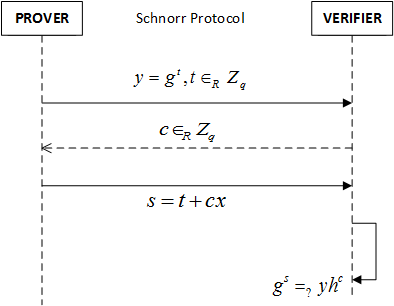
\includegraphics[width=1\textwidth]{schnorr.png}
\end{figure}
\end{columns}
\end{frame}

\begin{frame}[allowframebreaks]{Properties}

\begin{itemize}
\item \textbf{Completeness}
    \begin{center}
    $g^s = g^{t+cx} = g^t g^{cx} = yh^c \pmod{p}$
    \end{center}

\item \textbf{Soundness} 
Probability that \prv$^*$ cheats an honest verifier: $\frac{1}{q}$ - negligible - repeat to decrease
\pause
\item \textbf{Special soundness}
Let $(y,c,s)$ nad  $(y,c',s')$ be two successful protocol transcripts
\pause
\begin{align*}
 g^s = yh^c  \text{ και }  g^{s'} = yh^{c'}  \Rightarrow  g^s h^{-c}   = g^{s'} h^{-c'}  \Rightarrow \\
 g^{s-xc} = g^{s'-xc'} \Rightarrow  s-xc = s'-xc' \Rightarrow  
 x = \frac{c'-c}{s-s}
\end{align*}
\pause
Since \prv can answer these 2 questions he knows DLOG of $h$
\end{itemize}

\framebreak

\textbf{Zero knowledge}: \alert{no}
 
\begin{itemize}
\item A cheating verifier does not choose randomly  \pause
\item but bases each challenge to the commitment received before \siml \pause
\item In the simulated execution it will switch challenge \pause
\item \siml will not be able to respond \pause
\end{itemize}

How to add ZK: \pause

\begin{itemize}
\item \ver commits to randomness before the first message by  \prv or \pause
\item Challenge space $\{ 0 , 1 \} $ 
\begin{itemize}
\item In this case \ver has only two options. 
\item As a result the \siml can prepare for both.
\end{itemize} 
\end{itemize} 

\framebreak

It provides \green{Honest Verifier Zero Knowledge}. Let  \siml without knowledge of the witness $x$ and an honest \ver 
 
\begin{itemize}
\item \siml follows the protocol and commits to $y=g^t, t \in_R \zs{q}$
\item \ver selects $c \in_R \zs{q}$
\item If \siml can answer (which occurs with negligible probability) the protocol resumes normally  
\item Else the \ver is rewound (with the same random tape)  
\item \ver selects the same $c \in_R \zs{q}$ (because the random tape has not changed)  
\item \siml sends $s=t$. \ver will accept since $yh^{c} = g^t  h^{-c} h^{c} = g^t = g^s$ 
\end{itemize}
  
The conversations $(t \in_R \mathbb{Z}_q; g^t h^{-c}   , c \in_R \mathbb{Z}_q  , t )$ 
$(t,c \in_R \mathbb{Z}_q;  g^t  , c  , t+xc  )$
 follow the same distribution
\end{frame}
 

\begin{frame}{Removing interactivity}
\begin{block}{Question}
Can we do away with \ver?
\end{block}

\prv generates the proof by himself

The proof is verifiable by anyone

\begin{block}{Fiat Shamir Transform}
Replace the challenge with the output of a pseudorandom function on the commitment

In practice we use a hash function $\mathcal{H}$
\end{block}
\end{frame}

\begin{frame}{Non-interactive Schnorr with the Fiat Shamir}
\begin{block}{Input}
\begin{itemize}
\item \textbf{Public:} $g$ is a generator of an order $q$ subgroup of ( $\zs{p}$ with hard DLP and $h \in \zs{p}$ 
\item \textbf{Private:}\prv has a witness $x \in \zs{q}$ st: $h = g^x \bmod{p}$
\end{itemize}
\end{block}
\pause
The Prover:
\begin{itemize}
\item Randomly select $t \in_R \mathbb{Z}_{q}$,
\pause
\item Compute $y = g^t \bmod{p}$
\pause
\item \textbf{Compute $c = \mathcal{H}(y)$ where $\mathcal{H}$ is a hash function in $\mathbb{Z}_{q}$}
\pause

\item Compute $s=t+cx \bmod{q}$
\pause
\item \textbf{Release $(h,c,s)$}
\pause
\item \textbf{Anyone can verify that $c = \mathcal{H} (g^s h^{-c})$}
\end{itemize}
\end{frame} 

\begin{frame}{The common reference string}
Both parties have access to a string of random data

This is created in a trusted way (e.g. through a secure multiparty computation protocol)

The prover simulates the verifier challenge by selecting random data
\end{frame}

\subsection{Cryptography}

\begin{frame}{Homomorphic Encryption Schemes}
    Applying a function on the ciphertexts yields the encryption of a function on the plaintext
    \begin{align*}
    \enc(m_1) \otimes \enc(m_2) = \enc(m_1 \oplus m_2)
    \end{align*}
    Multiplicative Homomorphism in El Gamal:
    \begin{align*}
    \enc(m_1) \cdot \enc(m_2) = (g^{r_1},m_1 h^{r_1}) \cdot (g^{r_2},m_2 h^{r_2}) \\ = (g^{r_1 + r_2}, (m_1 \cdot m_2) h^{r_1 + r_2})
    \end{align*} 
    Additive Homomorphism in El Gamal:
    \begin{align*}
    \enc(m_1) \cdot \enc(m_2) = (g^{r_1},g^{m_1} h^{r_1}) \cdot (g^{r_2},g^{m_2} h^{r_2}) \\ = (g^{r_1 + r_2}, g^{m_1 + m_2} h^{r_1 + r_2})
    \end{align*} 
\end{frame}

\begin{frame}{Application - polynomials}
    \begin{block}{Task}
    Let $\enc(x) = g^x$ where $g$ is a suitable group generator and $p(x)=\sum_{i=0}^d a_i x^i$ a polynomial \\
    
    Two parties with knowledge of $x_0$ and $p(x)$ respectively can compute $\enc(p(x_0))$
    \end{block}

    \begin{itemize}
   
    \item The \ver (the party that knows $x_0$) releases 
    \begin{align*}\enc(x_0^0), \enc(x_0^1), \cdots, \enc(x_0^d)\end{align*} 
    into the common reference string
    \item The \prv (the party that knows the coefficients) computes:  
    \begin{align*}\prod_{i=0}^d \enc(x_0^i)^{a_i} = \enc(\sum_{i=0}^{d} a_i x_0^i) = \enc(p(x_0))  \end{align*} 

    \end{itemize}
\end{frame}

\subsubsection{Pairings}
\begin{frame}[allowframebreaks]{Pairings}
\begin{block}{In general}
Functions that map elements from source groups $\mathcal{G}_1,\mathcal{G}_2$ or $\mathcal{G}^2$ to a destination group $\mathcal G_T$.
\end{block}

\emph{What is interesting}: They transform difficult problems in $\mathcal G$ to easy problems in $\mathcal G_T$. 

\begin{block}{Definition}
A pairing is an efficiently calculable function $e : \mathcal G \times \mathcal G \rightarrow \mathcal G_T$ st:
\begin{itemize}
\item Bilinear: $e(g^a,g^b) = e(g,g)^{ab}$ where $g \in \mathcal G \ a,b \in \mathbb{Z}$
\item Non-Degenerate:If $\mathcal G=<g>$ then $\mathcal G_T = <e(g,g)>$
\end{itemize}
\end{block}

\framebreak

In practice: $G=\mathcal{E}(\mathbb{F}_p)$ and $G_T = \mathbb{F}_{p^a}$

\begin{block}{How to easily solve DDH}
Input: $(g, g^a, g^b, g^c)$

Check if $g^c = g^{ab}$

Easily compute $e(g^a, g^b) = e(g,g)^{ab}$

Compare with $e(g,g^c)=e(g,g)^c$

but the CDH remains hard
\end{block}

\begin{block}{Observation}
The pairing allows us to do a multiplication between 'encrypted' values
\end{block}
\end{frame}

\begin{frame}[allowframebreaks]{Application - check the correct evaluation of polynomials}
\begin{itemize}
    \item The \ver that knows $x_0$:
     \begin{itemize}
        \item computes and publishes into the CRS: \begin{align*} \enc(x_0^0), \enc(x_0^1), \cdots, \enc(x_0^d) \end{align*}
        \item selects a scaling factor $b$
        \item computes and publishes into the CRS: \begin{align*} \enc(bx_0^0), \enc(bx_0^1), \cdots, \enc(bx_0^d) \end{align*}
    \end{itemize} 
    \item The \prv that knows $p(x)$:
    \begin{itemize}
        \item computes and publishes $\enc(p(x_0)), \enc(bp(x_0))$
    
    \end{itemize}
    \item The secrets $b,x_0$ should be destroyed
\end{itemize}

\framebreak 
Check:
\begin{itemize}
    \item Use a pairing function $e$ to compute:
    \begin{itemize}
        \item $e(\enc(p(x_0)),\enc(b)) = e(g,g)^{bp(x_0)}$
        \item $e(\enc(bp(x_0)),\enc(1)) = e(g,g)^{bp(x_0)}$
    \end{itemize}
\end{itemize}
         
\begin{block}{Observation}
\begin{itemize}
    \item The homomorphic combination of encrypted polynomials allows us to do additions
    \item plus the multiplication from the pairing
\end{itemize}

\end{block}
\end{frame}

\begin{frame}{A 'new' security assumption}
    \begin{block}{Knowledge of exponents (Damgard 1991)}
    Let $\mathbb{G}$ a group of order $q$ generated by $g$ and $x \in_R \mathbb{Z}_q$. Let $h = g^x$
    
    For any adversary $\mathcal{A}(q,g,h)$ that outputs a value $(c,y)$ such that $y=c^x$,
    there exists an extractor $\mathcal{B}$ who on input $\mathcal{B}(q,g,h)$ 
    outputs $s$: $c=g^s$
    \end{block}
    \pause
    \begin{block}{Intuition}
        \begin{itemize}
            \item The exponent in question is $s$
            \item Since $y=c^x$ and we do not know $x$ the only way to have come up with $(c,y)$ is 
                  through $s$
            \item That is: $c=g^s$ and $y=h^s$
            \item Between ZKP of DLOG equality and double DLOG knowledge
            \item Non standard, but cannot be derived from standard assumptions such as the DDH.
        \end{itemize}
    \end{block}   
\end{frame}

\begin{frame}{KoE Relation to zk-Snarks}
There is no need to know $x$ in order to validate knowledge of exponent:
\begin{align*}
e(h,c) = e(g,y) = e(g,g)^{sx}
\end{align*}

\begin{block}{The correspondence}
$C=\enc(p(x_0))=g^{p(x_0)}$ and \\
$Y=\enc(bp(x_0))=g^{bp(x_0)}$
\end{block}
If it does not hold then a cheating prover might come up with $Y$ without knowing $p(x_0)$
\end{frame}

\begin{frame}{Remarks}
    \begin{itemize}
        \item Is it sound?
        \pause
        \item Answer: \emph{No} - the prover can cheat by replacing $p$ with \emph{any} polynomial
        \pause
        \item Is it zero knowledge?
        \pause
        \item Answer: \emph{No} - it allows the verifier to learn $\enc(p(x_0))$
    \end{itemize}
\end{frame}

\begin{frame}{Evaluate polynomials and check in ZK}
ZK: \ver must not even learn $\enc(p(x_0))$ 
\begin{itemize}
    \item \ver selects $b,x_0$ and computes:   \begin{align*}
        \enc(x_0^0),\enc(x_0^1),\cdots \enc(x_0^d)    \\
         \enc(bx_0^0),\enc(bx_0^1),\cdots \enc(bx_0^d) \end{align*}
    \item \prv selects $a$ and computes:  
        \begin{align*}
        \enc(a)\enc(p(x_0)) = \enc(a+p(x_0)) \\
        \enc(b)^a \enc(bp(x_0)) = \enc(ba)\enc(bp(x_0)) = \enc(b(a+p(x_0))))
        \end{align*}
    \item Check the pairing step as before:
        \begin{align*}
        e(\enc(a+p(x_0)),\enc(b))=e(g,g)^{b(a+p(x_0))} \\
        e(\enc(b(a+p(x_0))),\enc(1))=e(g,g)^{b(a+p(x_0))} 
        \end{align*}
\end{itemize}
\end{frame}

\begin{frame}{R1CS}

\begin{block}{Definition}
A system of rank-1 quadratic equations over $\mathbb{F}$ is a set of constraints $C  = \{ (\bm{a}_j, \bm{b}_j, \bm{c}_j) \}_{i=1}^{N_c} $ and $n \in \mathbb{N}$ where:
\begin{itemize}
    \item $\bm{a}_j,\bm{b}_j,\bm{c}_j \in \mathbb{F}^{1+N_v}$
    \item $n \leq N_v$
\end{itemize}
\end{block}

\begin{block}{Satisfiability}
A R1 system $C$ is satisfiable on input $\bm{x} \in \mathbb{F}^n$ if there is a witness $s \in \mathbb{F}^{N_v}:$
\begin{itemize}
    \item $\bm{x} = (s_1, \cdots, s_n)$
    \item $\forall j \in N_c:  \bm{a}_j \cdotp (1,\bm{s})  \times  \bm{b}_j \cdotp (1,\bm{s})  =  \bm{c}_j \cdotp (1,\bm{s})$
\end{itemize}
\end{block}  
\end{frame}

\begin{frame}{Facts}
\begin{block}{BC to R1CS}
Boolean circuit $C: \{0,1\}^n \times \{0,1\}^h \times \{0,1\}$ with $\alpha$ wires and $\beta$ (bilinear) gates 
$\rightarrow$
R1CS with with $N_v = \alpha$ and $N_c = \beta + h+1$
\end{block}

\begin{block}{AC to R1CS}
Arithmetic circuit $C: \mathbb{F}^n \times \mathbb{F}^h \times \mathbb{F}^l$ with $\alpha$ wires and $\beta$ (bilinear) gates 
$\rightarrow$
R1CS with with $N_v = \alpha$ and $N_c = \beta + l$
\end{block}
 
\end{frame}

\begin{frame}[allowframebreaks]{Quadratic Span Programs - QSP}

\begin{block}{Definition}
A QSP over a field $\mathbb{F}$ for inputs of length $n$ consists of
\begin{itemize}
    \item 2 sets of source polynomials: $\mathcal{V} = \{v_0, \cdots, v_m \}, \{ w_0, \cdots, w_m \}$
    \item the target polynomial: $t$
    \item an injective function $f : [n] \times \{0,1\} \rightarrow [m]$
\end{itemize}
\end{block}

\framebreak 
\begin{block}{QSP Verification}
An input $u \in \{0,1\}^n$ is accepted by a QSP iff $\exists$ tuples 
$a = (a_1, \cdots, a_m)$, $b = (b_1, \cdots, b_m) \in \mathbb{F}^m:$

\begin{itemize}
    \item $a_k \land b_k = 1$, if $\exists i: k=f(i,u_i)$
    \item $a_k \land b_k = 0$, if $\exists i: k=f(i,1-u_i)$
    \item $t$ divides the linear combination $v_a \cdot w_b$ where 
     $v_a = v_0+\sum_{i=1}^m a_i v_i$, \\
     $w_b = w_0+\sum_{i=1}^m b_i w_i$
\end{itemize}

\end{block}

\framebreak

Remarks: 

\begin{itemize}
    \item Check if a target polynomial divides a linear combination of some given polynomials
    \item $f$ restricts which polynomials can be used in the linear combination
    \item The NP witness are the $a,b$
    \item QSP Verification is NP-Complete 
    \item In practice:
    \begin{itemize}
        \item Find $h: th = v_a \cdot w_b \Leftrightarrow th - v_a \cdot w_b = \textbf{0}$       
        \item Check that it is a zero polynomial
        \item Evaluate at a single point $t(x_0)h(x_0) - v_a(x_0) \cdot w_b(x_0) = 0$ (The number of roots is tiny compared to the number of field elements)
     \end{itemize}
\end{itemize} 
\end{frame}

\begin{frame}[allowframebreaks]{Quadratic Arithmetic Programs}
\begin{block}{Definition}
A QAP $\mathcal{Q}$ over a field $\mathbb{F}$ is:
\begin{itemize}
    \item 3 sets of source polynomials $\mathcal{V} = \{v_0, \cdots, v_m \}$, $\mathcal{W} = \{ w_0, \cdots, w_m \}$, $\mathcal{Y}  = \{y_0, \cdots, y_m \}$
    \item the target polynomial $t$
    \item a function $f : \{0,1\}^n \rightarrow \{0,1\}^{n'}$
\end{itemize}
\end{block}

\framebreak

$\mathcal{Q}$ computes $f$ if:
 $ (c_1, \cdots ,c_{n+n'}) \in \mathbb{F}^{n+n'}$ is a valid assignment of
$f$’s inputs and outputs which happens
if and only if there exist coefficients $(c^{N+1},\cdots,c^m)$ such that $t(x)$ divides $p(x)$ where:
\begin{align*}
p(x) = (v_0(x)+\sum_{k=1}^m c_k v_k(x)) \cdot (w_0(x)+  \sum_{k=1}^m c_k w_k(x))\\ - (y_0(x)+\sum_{k=1}^m c_k y_k(x))
\end{align*}
 
\end{frame}

\section{The Proof}

\begin{frame}[fragile]{From Code to QAP}

\begin{block}{Process}
Code $\rightarrow$ Algebraic Circuit $\rightarrow$ R1CS 
$\rightarrow$ QAP $\rightarrow$ ZKSnark
\end{block}

\begin{python}
    def f(x): 
        y=x**3 
        return x+y+5   
\end{python}

\begin{block}{Task}
Prove that you executed f with input = $3$
\end{block}
\end{frame}

\begin{frame}[fragile]{Convert to circuit - Flattening}
    Convert code into a format that contains only commands of the form:
    \begin{itemize}
        \item \texttt{x=y}
        \item \texttt{x=y op z}  
    \end{itemize}
    
    As a result the function $f$ becomes:    
   \begin{python}
        def f(x): 
            sym_1 = x * x 
            y = sym_1 * x    
            sym_2 = y + x   
            out = sym_2 + 5
    \end{python}    
\end{frame}

\subsection{R1CS}
\begin{frame}{Convert to R1CS} 
\begin{block}{Rules}
    \begin{itemize}
        \item Each command can be considered as a logic gate and represented as a relation between vectors
        \item The vectors have as many elements as the total number of variables in the command plus one (for constants)
        \item Mapping vector $ [ one,  x,  out,  sym_1,  y,  sym_2 ] $
        \item Vector $\bm{c}$ is the left hand side
        \item Vector $\bm{a}, \bm{b}$ are the right hand sides
    \end{itemize}  
\end{block}

\end{frame}
 

\begin{frame}{Application to example commands}   
    \begin{columns}[T] % align columns
    \begin{column}{.48\textwidth}
        \begin{block}{Command}sym_1 = x * x\end{block}
        
        \begin{align*}        
             [ &one,&x,&out,&sym_1,&y,&sym_2 ]\\
             \bm{a} = [&0,&1,&0,&0,&0,&0]  \\
             \bm{b} = [&0,&1,&0,&0,&0,&0]  \\
             \bm{c} = [&0,&0,&0,&1,&0,&0] 
        \end{align*}
        
        Indeed $s = [1,3,0,9,0,0]$ satisfies: $\bm{s} \bigcdot \bm{a} \cdot \bm{s} \bigcdot \bm{b} - \bm{s} \bigcdot \bm{c} = 0$   
    \end{column}%
    \hfill%
    \begin{column}{.48\textwidth}
        \begin{block}{Command}y = sym1 * x\end{block}
        
        \begin{align*}        
              [ &one,&x,&out,&sym_1,&y,&sym_2 ]\\
             \bm{a} = [&0,&0,&0,&1,&0,&0]  \\
             \bm{b} = [&0,&1,&0,&0,&0,&0]  \\
             \bm{c} = [&0,&0,&0,&0,&1,&0] 
        \end{align*}    
\end{column}%
\end{columns} 
\end{frame}

\begin{frame}{Application to commands}   
    \begin{columns}[T] % align columns
    \begin{column}{.48\textwidth}
    \begin{block}{Command}sym2 = y+x\end{block}
    
    \begin{align*}       
         [ &one,&x,&out,&sym_1,&y,&sym_2 ]\\ 
         \bm{a} &= [&0,&1,&0,&0,&1,&0]  \\ 
         \bm{b} &= [&1,&0,&0,&0,&0,&0]  \\
         \bm{c} &= [&0,&0,&0,&0,&0,&1] 
    \end{align*}    
    Remark: addition is implied in the dot product
    \end{column}%
    \hfill%
    \begin{column}{.48\textwidth}
    \begin{block}{Command}out = sym2+5\end{block}
    
    \begin{align*}     
         [ &one,&x,&out,&sym_1,&y,&sym_2 ]\\    
         \bm{a} = [&5,&0,&0,&0,&0,&1]  \\
         \bm{b} = [&1,&0,&0,&0,&0,&0]  \\
         \bm{c} = [&1,&0,&0,&0,&0,&0] 
    \end{align*}    
    \end{column}%
\end{columns} 
\end{frame}

\begin{frame}{The final R1CS}
    \begin{align*}        
         \bm{A} = \{[0,1,0,0,0,0], [0,0,0,1,0,0],[0,1,0,0,1,0],[5,0,0,0,0,1]  \}\\
         \bm{B} = \{[0,1,0,0,0,0],[0,1,0,0,0,0],[1,0,0,0,0,0] ,[1,0,0,0,0,0]  \}\\
         \bm{C} = \{[0,0,0,1,0,0], [0,0,0,0,1,0], [0,0,0,0,0,1] ,[1,0,0,0,0,0]  \}
    \end{align*}  
    The execution is the vector  $\bm{s} = [1,3,35,9,27,30] $
\end{frame}

\subsection{QSP}
\begin{frame}{From Vectors To Polynomials}
    \begin{block}{Why?}
        Because we can check all the constraints simultaneously!
    \end{block}
    \begin{itemize}
        \item Use Lagrange interpolation to transform the sets of $m$ vectors with $n$ elements into $n$ polynomials of degree $m-1$
        \item Construct polynomial $a_j(i) =A[i][j]$ (value element of vector $i$ in position $j$)
        \item For instance: $a_1(1) = 0, a_1(2) = 0, a_1(3)=0, a_1(4) = 5$
        \item $a_1(x) = \frac{5}{6}x^3-5x^2+\frac{55}{6}x-5$ or in vector form $\bm{a}_1 = [-5,\frac{55}{6},-5,\frac{5}{6}]$
        \item Repeat for $\bm{B}, \bm{C}$
        \item Compute $t = A \cdot s \times B \cdot s - C \cdot s$
        \item Compute $h$ from $t,A,B,C$ using FFT 
        \item Compute $a_i, b_i$ from the input
    \end{itemize}
\end{frame}
 

\subsection{zkSNARK}
\begin{frame}[allowframebreaks]{Setup Phase} 
    \begin{itemize}
        \item Public verifiability
        \item Non interactive
        \item Fix the homomorphic encryption scheme, verifier, polynomials 
        \item \ver selects random field elements $x_0,b \in \mathbb{F}$
        \item computes and publishes in the CRS:
        \begin{itemize}
            \item $\{ \enc(x_0^k) \}_{k=0}^d$
            \item $\{ \enc(bx_0^k)\}_{k=0}^d$
            \item $\{ \enc(v_k(x_0)),\enc(bv_k(x_0)) \}_{k=1}^m$
            \item $\{ \enc(w_k(x_0)),\enc(bw_k(x_0)) \}_{k=1}^m$
            \item $\{ \enc(y_k(x_0)),\enc(by_k(x_0)) \}_{k=1}^m$
            \item $\enc(t(x_0)), \enc(bt(x_0))$
        \end{itemize} 

        \framebreak

        \item selects random field values $\gamma, \beta_v, \beta_w, \beta_y$ in order to ensure soundness (i.e. that the correct polynomials were evaluated)
        \item computes and publishes in the CRS:
        \begin{itemize}
            \item $\enc(\gamma), \enc(\beta_v \gamma), \enc(\beta_w \gamma), \enc(\beta_y \gamma)$
            \item $\{ \enc( \beta_v v_k(x_0))\}_{k=1}^m$
            \item $\{ \enc(\beta_w w_k(x_0))\}_{k=1}^m$
            \item $\{ \enc(\beta_y y_k(x_0))\}_{k=1}^m$
            \item $\enc(\beta_v t(x_0)), \enc(\beta_w t(x_0)), \enc(\beta_y t(x_0))$
        \end{itemize} 

        All computations in the proof must use only these elements
    \end{itemize}
\end{frame}

\begin{frame}{The prover}
\begin{itemize}
    \item Evaluates the circuit for the function and obtains the output
    \item As a result the \prv knows the values of $c_i$
    \item Solves for $h$
    \item Define:
    \begin{itemize}
        \item $I_{mid}$: the indices that are not in the image of $f$
        \item $v_{mid}(x) = \sum_{k \in I_{mid}} c_k v_k(x)$
    \end{itemize}
    \item Generate the proof (9 encrypted values):
    \begin{itemize}
        \item $V_{mid} = \enc(v_{mid}(x_0))$, $W = \enc(w(x_0))$, 
        $Y=\enc(y(x_0))$, $H = \enc(h(x_0))$
        \item $V_{mid}^{'} = \enc(b v_{mid}(x_0))$, $W^{'} = \enc(b w(x_0))$, $Y^{'}=\enc(by(x_0))$, $H^{'} = \enc(bh(x_0))$
        \item $K = \enc(\beta_v v_{mid}(x_0) + \beta_w w(x_0)+\beta_y y(x_0)) $
    \end{itemize}
    \item All these values can be computed by leveraging the homomorphic properties of the underlying cryptosystem from what is on the CRS 
\end{itemize}
\end{frame}

\begin{frame}{The verifier}
\begin{itemize}
    \item Computes $I_{mid}$ from the input $u$
    \item Computes $\enc(v_{io}(x_0)) = \enc(\sum_{k \notin I_{mid}} c_k v_k(x_0))$
    \item Verifies the following equations using the pairing function:
    \begin{itemize}
        \item $e(V_{mid}^{'},\enc(1)) = e(V_{mid},\enc(b))$ 
        \item $e(W^{'},\enc(1)) = e(W,\enc(b))$,
        \item $e(H^{'},\enc(1)) = e(H,\enc(b))$
        \item $e(Y^{'},\enc(1)) = e(Y,\enc(b))$
        \item For soundness check:\\
        $e(\enc(\gamma),K) = e(\enc(\beta_v \gamma),V_{mid}) \cdot e(\enc(\beta_w \gamma),W) \cdot e(\enc(\beta_y \gamma),Y)$  
        \item Check the QAP relation:\\
        $\frac{e(\enc(v_0(x_0))\cdot \enc(v_{in}(x_0)) \cdot V_{mid},\enc(w_0(x_0)W))}{e(y_0(x_0)Y,\enc(1))} = e(H,\enc(t(x_0))$  
    \end{itemize}
\end{itemize}
\end{frame}

\begin{frame}{Completeness}
\small
\begin{flalign*}
    e(\enc(\gamma),K) = 
    \\ e(\enc(\gamma),\enc(\beta_v v_{mid}(x_0) + \beta_w w(x_0) + \beta_y y(x_0))) = 
    \\ e(g^{\gamma}, g^{\beta_v v_{mid}(x_0)+\beta_w w(x_0) + \beta_y y(x_0)}) =
    \\ e(g,g)^{\gamma \cdot (\beta_v v_{mid}(x_0) + \beta_w w(x_0) + \beta_y y(x_0))}
\end{flalign*}

\begin{flalign*}  
    e(\enc(\beta_v \gamma),V_{mid}) \cdot  e(\enc(\beta_w \gamma),W) \cdot  e(\enc(\beta_y \gamma),Y) = 
    \\ e(\enc(\beta_v \gamma,\enc(v_{mid}(x_0))) e(\enc(\beta_w \gamma),\enc(w(x_0))) e(\enc(\beta_y \gamma),\enc(y(x_0))) = 
    \\ e(g,g)^{\beta_v \gamma v_{mid}(x_0)} \cdot e(g,g)^{\beta_w \gamma w(x_0)} \cdot e(g,g)^{\beta_y \gamma y(x_0)}= 
    \\ e(g,g)^{\beta_v \gamma v_{mid}(x_0)+\beta_w \gamma w(x_0)+\beta_y \gamma y(x_0)}
\end{flalign*}
\end{frame}

\begin{frame}[allowframebreaks]{Completeness for the QAP Relation}
The parts of the left hand pairings:
\begin{align*}
\small
\enc(v_0(x_0)) \enc(v_{in}(x_0)) V_{mid} = \\
\enc(v_0(x_0)) \enc(v_{in}(x_0)) \enc(v_{mid}(x_0)) = \\
\enc(v_0(x_0) + v_{in}(x_0) + v_{mid}(x_0)) = \\ 
\enc(v_0(x_0)+\sum_{i=1}^m c_i v_i(x_0)) = \enc(v(x_0))
\end{align*}

\begin{align*}\small
\enc(w_0(x_0))W= 
\enc(w_0(x_0))\enc(w(x_0))=\\
\enc(w_0(x_0)+\sum_{i=1}^m(c_i w_i(x_0)))=\enc(w(x_0))
\end{align*}

\begin{align*}\small
\enc(y_0(x_0))Y= 
\enc(y_0(x_0))\enc(y(x_0))=\\
\enc(y_0(x_0)+\sum_{i=1}^m(c_i y_i(x_0)))=\enc(y(x_0))
\end{align*}

\framebreak
Left hand side:
\begin{align*}
e(\enc(v_a(x_0)),\enc(w_b(x_0)))=e(g,g)^{v(x_0) \cdot w(x_0) - y(x_0)}
\end{align*}
Right hand side:
\begin{align*}
e(H,\enc(t(x_0)))=e(g^h(x_0),g^t(x_0))=e(g,g)^{h(x_0)t(x_0)}
\end{align*}
\end{frame}

\begin{frame}{Intuition between soundness}
The relation 
$e(\enc(\gamma),K) = e(\enc(\beta_v \gamma),V_{mid}) \cdot e(\enc(\beta_w \gamma),W) \cdot e(\enc(\beta_y \gamma),Y)$
protects from a prover that tries to cheat by using another polynomial.
\begin{itemize}
    \item The values $\beta_v, \beta_w, \beta_y$ do not appear in the CRS in isolation
    \item The expression $\beta_v v_{mid}(x_0) + \beta_w w(x_0))+\beta_y y(x_0) $ can only be encrypted from the respected values in the CRS in encrypted form mixed with $\gamma$
\end{itemize}
\end{frame}

\begin{frame}{Shifting for Zero Knowledge}
The \prv chooses $\delta_{mid}, \delta_w, \delta_y$. \\
Define 
\begin{itemize}
\item $V_{\delta{mid}} = \enc(v_{mid}(x_0)+\delta_{mid}t(x_0))$
\item $w_{\delta}(x_0) = w(x_0)+\delta_w t(x_0)$
\item $y_{\delta}(x_0) = y(x_0)+\delta_y t(x_0)$
\item As a result $V_{mid}$, $W$, $Y$ are randomised
\end{itemize}
The equation $v(x_0)w(x_0)-y(x_0)= h(x_0)t(x_0)$ must still hold

To achieve this we replace $H = \enc(h(x_0))$ in the CRS accordingly

\end{frame}

\begin{frame}{vnTinyRAM}
\begin{itemize}
    \item zk-SNARKs for a general purpose CPU
    \item Circuit generator: Translate program execution into sequence of circuits
    \item Compose zk-SNARKs for these circuits
    \item Bound on the running time
\end{itemize}
\end{frame}

\section{Applications}

\subsection{Verifying cloud computations}
\begin{frame}[allowframebreaks]{Pinnochio: A cloud based lie detector}
\begin{itemize}
    \item General purpose computation validator
    \item Client: represents functions as a public evaluation key
    \item Client: provides input or ZKPoK of some property of the input
    \item Server: evaluates the computation and provides proof (signature)
    \item Compiler toolchain to use with C-programs
    \item Transforms to QAP, QSP
    \item Use:
    \begin{itemize}
        \item Protect against malicious servers
        \item Extra server feature (at a higher price)
    \end{itemize}
    \item Performance
    \begin{itemize}
        \item Setup: Linear in the size of the computation
        \item Proof Size: constant (288 bytes)
    \begin{itemize}
        \item Does not depend on function
        \item Does not depend on input/output size
    \end{itemize}
        \item Verification: Linear in the size of the input and output typically 10ms (5 - 7 orders of magnitude gain)
        \item Proof generation: up to 60 times fewer work
    \end{itemize}
    %\includegraphics
\end{itemize}
\end{frame}

\subsection{zCash}
\begin{frame}[allowframebreaks]{Bitcoin's problem}
    Bitcoin is not anonymous
    \begin{itemize}
        \item All transactions are recorded in the blockchain
        \item Users use pseudonyms
        \item Deanonymization
        \begin{itemize}
            \item The structure of the transaction graph
            \item Real world information (value, dates, blockchain exit points) 
        \end{itemize} 
    \end{itemize}
    Bitcoins are not fully fungible
    \begin{itemize}
        \item In the protocol itself all coins have the same value
    \end{itemize}
    
    but...
    \framebreak

   
    \begin{itemize}
        \item Each coin has a history than can be traced
        \item This might have an effect on the ability to spend the coins or on their value (e.g. Wanacry ransomware)
    \end{itemize}

    A first solutions: mixes
    \begin{itemize}
        \item Users entrust their coins to a 'trusted' entity
        \item They receive coins with the same value but different origins
        \item Many problems (fees, delays, trust)
    \end{itemize}
\end{frame}

\begin{frame}{ZeroCoin}
    \begin{itemize} 
    \item A decentralised mix
    \item Two kinds of coins: base and anonymous
    \item Each anonymous transaction is accompanied by a ZK proof that the coin spent can be linked to a valid base coin
    \begin{itemize} 
        \item The base coin comes from a valid transaction
        \item The base coin is unspent
    \end{itemize}
    \item Problems:
        \begin{itemize}
            \item Performance bottleneck for ZK proofs
            \item Functionality: Does not support all denominations etc.
            \item Anonymity: Does not hide metadata
        \end{itemize}
    \end{itemize}
    \item Transactions occur using the base coin and are periodically washed in the distributed mix
\end{frame}

\begin{frame}{zCash=Zerocoin+SNARKs}
    \begin{itemize}
        \item Performance
        \begin{itemize}
            \begin{itemize}
                 \item 288 byte proof
                 \item 895MB CRS
                 \item transaction < 1KB (vs 45KB in Zerocoin)
                 \item 6ms verification (vs 450ms in Zerocoin)
                 \item 1min to make a transaction
            \end{itemize}
        \end{itemize}
    \end{itemize}
\end{frame}

\begin{frame}[allowframebreaks]{zCash CRS generation ceremony}
    \begin{block}{Goal}
        \begin{itemize}
            \item Generate $x_0$ in CRS: $g^{x_0^1}, \cdots, g^{x_0^d}$
            \item No participant must learn the entire $x_0$
            \item All shares of $x_0$ must be later destroyed
            \item A single honest participant is required
        \end{itemize}
    \end{block}
    \framebreak
    \begin{block}{The protocol}
        \begin{itemize}
            \item Each participant generates a random $s_i$
            \item The first participant computes and publishes $g^{s_1}, \cdots, g^{s_1^d}$  
            \item The second partipant computes $g^{s_1 \textbb{s_2}}, \cdots, g^{s_1^d \textbb{s_2}^d}$
            \item $\cdots$
            \item The last participant computes $g^{s_1 s_2 \cdots \textbb{s_n}}, \cdots, g^{s_1^d s_2^d \cdots \textbb{s_n}^d}$
            \item $x_0 = s_1 s_2 \cdots \textbb{s_n}$
        \end{itemize} 
    \end{block}
    \framebreak
    \begin{block}{Validation}
         A partipant might cheat by computing $g^{s_p \cdot s_i^`}$. validation can be done using pairings.
         \begin{itemize}
            \item $e(g^{s_i},g^{s_i})=e(g,g)^{s_i^2}$
            \item $e(g,g^{s_i^2})=e(g,g)^{s_i^2}$
         \end{itemize}
         This check is repeat for all powers
    \end{block}
\end{frame}


\section{References}
\begin{frame}{Bibliography-References}
\begin{tiny}
\begin{enumerate}
\item Rosario Gennaro Craig Gentry Bryan Parno Mariana Raykova "Quadratic span programs and succinct NIZKs without PCPs." Annual International Conference on the Theory and Applications of Cryptographic Techniques. Springer Berlin Heidelberg, 2013.
\item Parno, B., Howell, J., Gentry, C., & Raykova, M. (2013, May). Pinocchio: Nearly practical verifiable computation. In Security and Privacy (SP), 2013 IEEE Symposium on (pp. 238-252). IEEE.
\item Eli Ben Sasson, Alessandro Chiesa, Christina Garman, Matthew Green, Ian Miers, Eran Tromer, and Madars Virza. 2014. Zerocash: Decentralized Anonymous Payments from Bitcoin. In Proceedings of the 2014 IEEE Symposium on Security and Privacy (SP '14). IEEE Computer Society, Washington, DC, USA, 459-474. 
\item Eli Ben-Sasson, Alessandro Chiesa, Eran Tromer, and Madars Virza. "Succinct Non-Interactive Zero Knowledge for a von Neumann Architecture." In USENIX Security, vol. 2014. 2014.
\item I. Damgård. Towards practical public-key cryptosystems provably-secure against chosen-ciphertext attacks. Advances in Cryptology – CRYPTO ’91, Lecture Notes
in Computer Science Vol. 576, J. Feigenbaum ed., Springer-Verlag, 1991.
\item \href{http://www.scipr-lab.org/}{Succinct Computational Integrity and Privacy Research}
\item Christian Reitwiessner \href{https://blog.ethereum.org/2016/12/05/zksnarks-in-a-nutshell/}{zkSNARKs in a nutshell}
\item Vitalik Buterin \href{https://medium.com/@VitalikButerin/zk-snarks-under-the-hood-b33151a013f6}{zkSNARKs: under the hood}
\item Alfred Menezes \href{https://www.math.uwaterloo.ca/~ajmeneze/publications/pairings.pdf}{An introduction to pairing based crypto}
\item \href{https://z.cash/technology/paramgen.html}{Zerocash parameter generation}
\end{enumerate}
\end{tiny}
\end{frame}

\end{document}
